\documentclass[12pt,A4, onecolumn]{exam}
\usepackage{amsmath}
\usepackage{amssymb}
\usepackage{listings}
\usepackage{xcolor}
\usepackage[lmargin=40pt, tmargin=0.8in]{geometry}  %For centering solution box
\lhead{TEK4090 -- Introduction to Modern Control\\}
\rhead{Assignment 1\\}
% \chead{\hline} % Un-comment to draw line below header
\thispagestyle{empty}   %For removing header/footer from page 1

\usepackage{graphicx}
\graphicspath{{../../figs/}}

\def\showsoln{1}

\begin{document}

\begingroup  
    \centering
    \LARGE TEK4090 -- Introduction to Modern Control\\
    \LARGE Assignment 1\\[0.5em]
    \large Due: September 18 2025, 13:15\\
\endgroup
\rule{\textwidth}{0.4pt}
%\pointsdroppedatright   %Self-explanatory
\printanswers


\renewcommand{\solutiontitle}{\noindent\textbf{Ans:}\enspace}   %Replace "Ans:" with starting keyword in solution box

\begin{questions}

  \question[10] Suppose that $v_1,\dots,v_m$ is linearly independent in $V$, and that $w\in V$. Show that
    \begin{align}
      v_1,\dots,v_m, w \text{ is linearly independent } \iff w\notin \mathrm{span}(v_1,\dots,v_m).
    \end{align}


  \begin{solution}
    I will show that $ i) \rightarrow ii) $ and then that $ ii) \rightarrow i) $ 
    
    Assume $ v_1, ... , v_m, w $ is lin. indep.
    
    Pf by contradiction:

    \begin{align*}
      w \in span(v1, ..., v_m) \\
       w &= \alpha_{1}^{} v_1 + ... + \alpha_{m}^ {} v_m  \\
       0 &= \alpha_{1}^{} v_1 + ... + \alpha_{m}^ {} v_m  + (-1) w\\
    \end{align*}

    This contradicts that $ v_1, ..., v_m, w $ is linearly independent, because for any combination of indep. vectors, they must equal if and only if all coefficients $ \alpha_{1}^{} , ..., \alpha_{m}^{} = 0  $. This contradicts independence, since a non-trivial linear combination gives 0. Hence, $ w \notin span(v_1, ..., v_m) $    

    will now prove that $ ii) \rightarrow i) $. Will also use proof by contradiction. Assume that $ w \in span(v_1, ..., v_m) $. This means that w can be written as a linear combination of the vectors in $ span(v1, ..., v_m) $ 

    \[
       w = \alpha_{1}^{} v_1 + ... + \alpha_{m}^{} v_m
    \]

    This means that by definition, the list $ (v_1, ..., v_m, w) $ is dependent, and this is our contradiction.
    Thus, for $ v_1, ..., v_m, w $ to be independent, $ w \notin span(v_1, ..., v_m)$ has to be true  

  \end{solution}

  \question[10] Let $A,B\in \mathbb{R}^{n\times n}$, and define the \emph{trace} of $A$ as $\mathrm{tr}(A)=\sum_{i=1}^n A_{ii}$. Show that 
    \begin{align}
      \dfrac{d \mathrm{tr}(AB)}{dA} = B^T.
    \end{align}
    Hint: Find $\frac{d\mathrm{tr}(AB)}{dA_{ij}}$.


    \begin{solution}
      \begin{align*}
        tr(AB) &= \sum_{ n }^{ i=1 } (AB)_{i, i} \\
        &= \sum_{ n }^{ i } \sum_{ n }^{ j } A_{i, j}B_{j, i}
      \end{align*}

      Thus we get that  

      \begin{align*}
        \frac{dtr(AB)} {dA_{i,j}} \\
        &= \frac{d(\sum_{ n }^{ i } \sum_{ n }^{ j } A_{i, j} B_{j, i})} {dA_{i, j}} \\ 
        &= B_{j, i}
      \end{align*}

      And if we now replace $ A_{i, j} $ with $ A $ in the denominator, we get
      
      \[
         \frac{d(\sum_{ n }^{ i } \sum_{ n }^{ j } A_{i, j} B_{j, i})} {dA} = B^T
      \] 
      
    \end{solution}

  \question[15] Suppose that $T:V\mapsto V$ is a linear map, and suppose that $S:V\mapsto V$ is an invertible linear map.
    \begin{parts}
      \part Prove that $T$ and $S^{-1}TS$ have the same eigenvalues
      \part Describe the relationship between the eigenvectors of $T$ and the eigenvectors of $S^{-1}TS$.


      \begin{solution}
        We want to prove that 

        \[
           T(v)=\lambda v = S^{-1}TS(v)
        \]  
        Matrix multiply both sides by $ S $ and get
        \[
           ST(v) = S(\lambda v) = SS^{-1}TS(v)
        \]
        \[
          SS^{-1}TS(v) = ITS(v) 
        \] 
        \[
           T(S(v)) = \lambda S(v)
        \] 
        where $ I $ is the identity matrix 

        Since S is a linear invertible map, we get that $ S
        (\lambda v) = \lambda S(v)$ 


        Now we set $ v = S^{-1}(w) $ and $ T(w) = \lambda w$
        
        Then we have that $ S(v) = w $
        
        \begin{align*}
          S^{-1}TS(v) &= S^{-1}T(w) \\
          S^{-1}(\lambda w) &= \lambda S^{-1}(w) \\
          &= \lambda v 
        \end{align*}
        
        which is what we wanted to prove; namely that $ T $ and $ S^{-1}TV $ are similar, and thus have simialr eigenvalues. This is correct assuming the maps $ T $ is linear and that $ S $ is linear and invertible     
      \end{solution}
    \end{parts}

\question[30] Consider the feedback block diagram:
  \begin{center}
    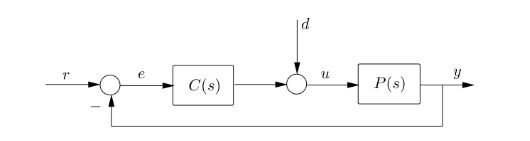
\includegraphics[width=0.75\linewidth]{Figures/feedback_block_diagram.png}
  \end{center}
\begin{parts}
  \part Find the transfer function from $d$ to $y$.

  \begin{solution}
    
  
    The transfer function $ T(s)=\frac{Y(S)} {D(S)} $ where
    
    \begin{itemize}
      \item $ Y(S)=P(s) \left( C(s)+D(s) \right)$
      \item $ C(s)=U(s)E(s) $
      \item $ E(s)=R(s)-Y(s) $   
    \end{itemize}

    We are not interested in the error, so we set the reference to 0. 

    \begin{align*}
      Y(s)&=P(s) U(s) + P(s)D(s) \\
      &= P(s) \left[ -Y(s)C(s) \right] P(s)D(s) \\
      Y(s) \left[1+P(s)C(s) \right] &= P(s)D(s) \\
      \frac{Y(s)} {D(s)} &= \frac{P(s)} {1+P(s)C(s)}  
    \end{align*}



  \end{solution}

  \part Suppose the plant has transfer function
\begin{align}
  P(s) = \dfrac{(s+1)}{s^2-4s+13}
\end{align} 


What are the poles of $P(s)$? What can you infer about the stability of the (open-loop) plant $P(s)$?

\begin{solution}
  We have an unstable open-loop plant, if at least one root of the denominator is located in the RHP. For $ P(s) = \frac{N} {D}  $, we have
  
  \[
     s^2-4s+13 = 0
  \] 

  In the abc formula, this gives 
  \[
     2 \pm j 3
  \] 

  Since the real part of both roots are $ > 0 $, we have instability of the plant $ P(s) $.  
\end{solution}

  \part Suppose $C(s)$ is given by 
    \begin{align}
      C(s) = \dfrac{1}{s}
    \end{align}
    Does $C(s)$ stabilize the feedback system?  

    \begin{solution}
      To find this out if controller $ C(s) $ stabilizes the system, I find the roots of the characteristic equation 

      \[
         1 + C(s)P(s)=0
      \] 

      If 

      \begin{itemize}
        \item $ C(s) = \frac{C_n} {C_d} $
        \item $ P(s) = \frac{P_n} {P_d} $  
      \end{itemize}

      I can formulate algebraically the new equation 

      \[
         C_d * P_d + C_n * P_n = 0
      \] 

      In matlab, this gives the following roots

      \begin{itemize}
        \item $ 2.0350 + 3.1849i $
        \item $ 2.0350 - 3.1849i $
        \item $ -0.0700 + 0.0000i $ 
      \end{itemize}

      This confirms that $ C(s) $ does not indeed stabilize the feedback system
      
      Here is the script I used:

      \begin{verbatim}
        nC = [1];
        dC = [1,0];

        nP= [1,1];
        dP = [1,-4,13];

        numProd = conv(nD, nC);
        denProd = conv(dC, dD);

        ml = max(length(denProd), length(numProd));
        denProd_padded = [zeros(1, ml - length(denProd)), denProd];
        numProd_padded = [zeros(1, ml - length(numProd)), numProd];

        char_poly = denProd_padded + numProd_padded;

        r = roots(char_poly);
        disp(r)
      \end{verbatim}

    \end{solution}
  \part \label{1} Now, suppose the plant and controller are given by
    \begin{align}
      P(s) = \dfrac{10}{(s+1)},~C(s) =\dfrac{K}{s}.
    \end{align}
  Find the values of $K$ for which the feedback loop is stable.

  \begin{solution}
    We are now given a gain K, and we will have to find the interval of K that makes the feedback system stable where $ P(s) = \frac{10} {s+1} $ and $ C(s)= \frac{K} {s}  $  

    Numerically, I have written a script that defines K as an array of equally spaced points, decided by a discretization step, that increases accuracy the higher it is.

    I get from my numeric estimation that for all $ 0 < K $, the system becomes stable. The following graph shows a parametrization of this fact, where the gain K is plotted on the x-axis, and stability is true $ (=1) $ if K gives stability, and 0 otherwise
    
    Its a step function of sorts
    \[
       y(K) = \begin{cases}
        1& \text{if K gives stability}\\
        0& \text{otherwise}
       \end{cases}
    \] 

    \begin{center}
      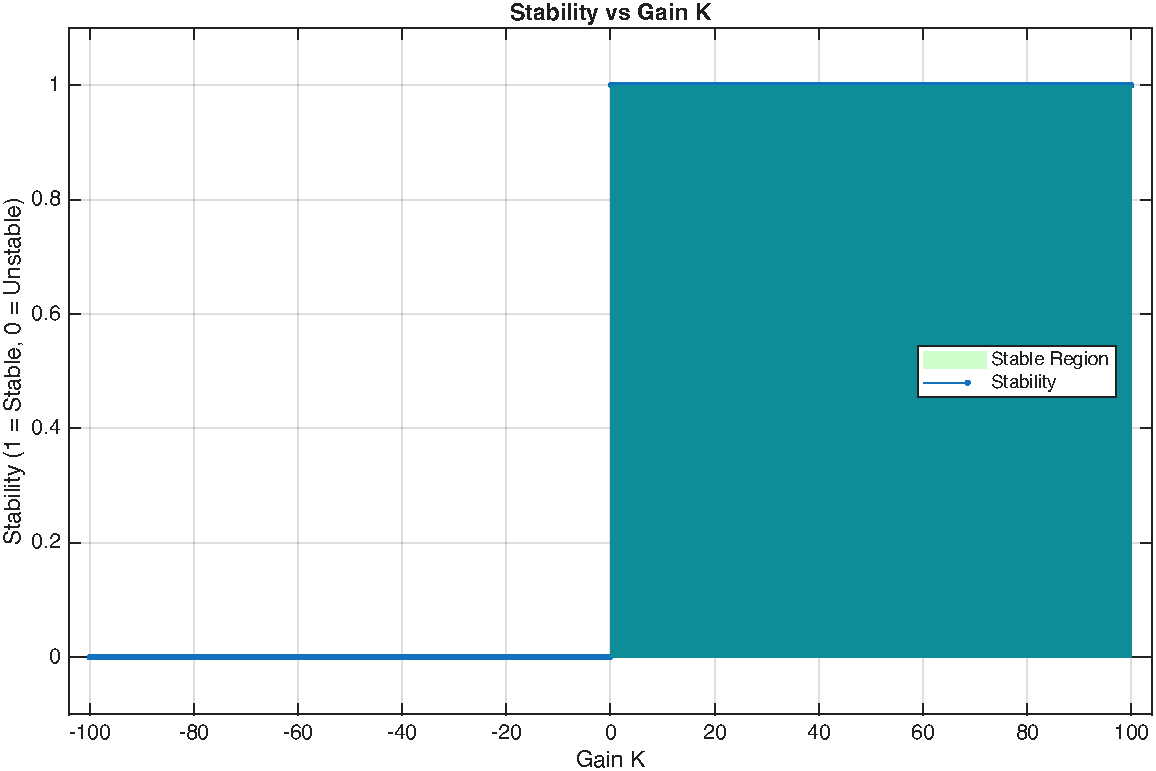
\includegraphics[width=0.75\linewidth]{Figures/stability_plot.pdf}
    \end{center}

    This can also be solved analytically by taking the transfer function, put in the new $ P(s) $ and $ C(s) $ and solve 
    
    \begin{align*}
      \frac{P(s)} {1+P(s)C(s)} &= \frac{\frac{10} {s+1}} {1 + \frac{10K} {s^2+s} }  \\
      &= \frac{(s^2+s) \frac{10} {s+1} } {s^2+s+10K} 
    \end{align*}

    In the abc-formula, this becomes 

    \[
       \frac{-1 \pm \sqrt{1-40K}} {2} 
    \] 
    If $ K=0 $ this gives that $ s=0 $ and $ s=-1/2 $ which gives marginal stability, and for $ K<0 $, it gives that s has positive roots. so $ K>0 $ gives stability, which is justified by the graph.
    
    The key insight is that K adds phase lag, improving steady state performance
  \end{solution}

  \part Fix a value of $K$ such that the system in part~(\ref{1}) is stable, and suppose the system is subject to a disturbance $D(s) = 100$. What will the final value of $y$ be?

  \begin{solution}
    To solve this, we state the final value theorem.

    \[
       lim_{t\rightarrow \infty} y(t) = lim_{s \rightarrow 0} sY(s)
    \] 

    we have that 
    \[
       Y(s) = \frac{C(s)P(s)} {1+P(s)C(s)}R(s) + \frac{P(s)} {1+P(s)C(s)} D(s)  
    \] 

    We set $ R(s) =0$ because we dont care about reference when we allow for external disturbances in this case, because we want to examine how disturbances affects our equilibrium state. We also set $ D(s) = \frac{100} {s}  $ because it is a step function, and $ d=100 $   transformed to the laplace domain, we have that $ D(s)=\frac{100} {s}  $   
    
    so we have 

    \begin{align*}
      lim_{t \rightarrow \infty} s \frac{\frac{10} {1+s} } {1+\frac{10K} {s(s+1)} } * \frac{100} {s}  &= lim_{t \rightarrow \infty} \frac{1000s} {s^2+s+10K} \\
      &= 0 
    \end{align*}

    
  \end{solution}
\end{parts}

    

\question[10] Consider the standard feedback system with
\begin{align}
C(s) = K,~
P (s) =\dfrac{
s^2 + 1}{
(s^2 + 2)(s - 2)}
\end{align}
\begin{parts}
  
\part Sketch the Nyquist plot of $P (s)$. Include correct asymptotes to infinity and to the origin.

\begin{solution}
  Include the figure for the nyquist plot for P(s)

  \begin{center}
      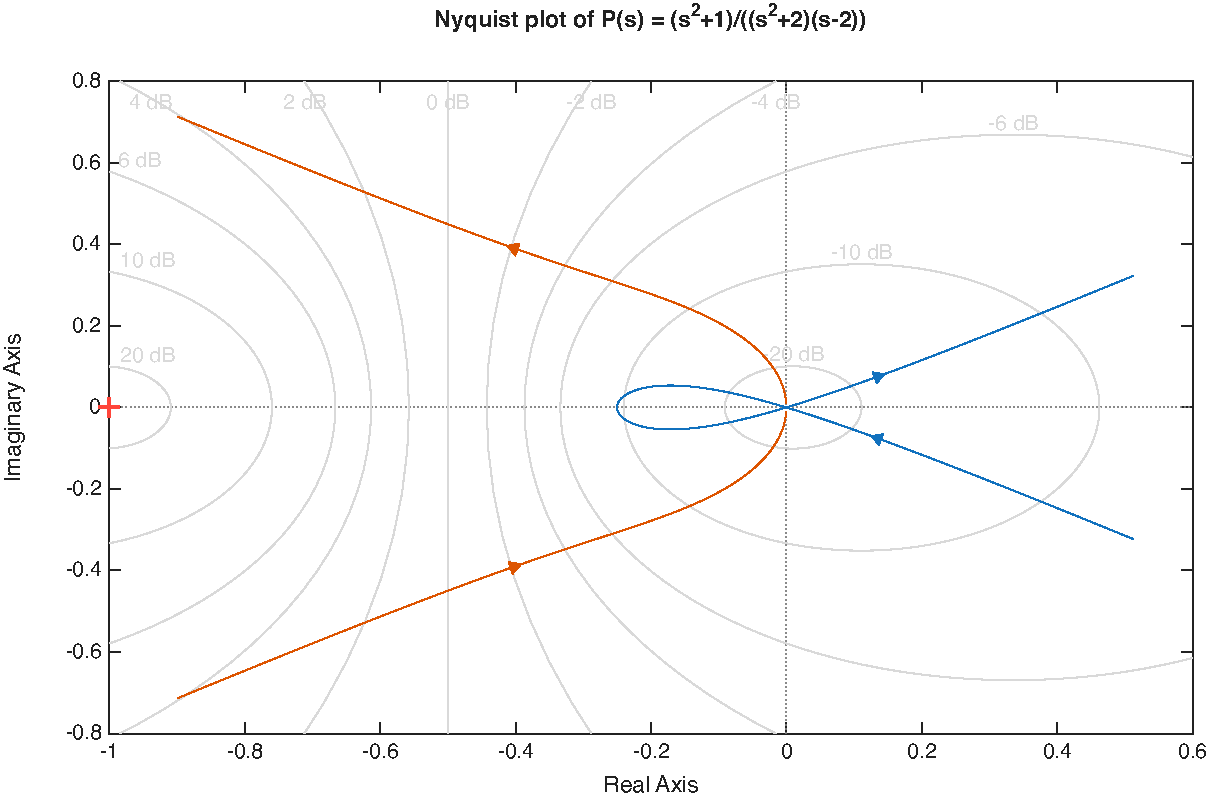
\includegraphics[width=0.75\linewidth]{Figures/nyquist_fiveA.pdf}
  \end{center}
\end{solution}

\part Indicate the number of encirclements (and their orientations) of all possible critical points.

\begin{solution}
  To indicate the number of encirclements, I want to talk about the Principle of the argument

  From Classical Control (Francis), its stated that when the characteristic polynomial has no right hand poles (RHP), then the system is stable. It can be shown that for a feedback system like we are dealing with now, the characteristic polynomial is equal to

  \[
     1 + KP(s) = 0
  \] 

  Since $ C(s) = K $ where K is the gain. The loop gain is defined as the sum of the gain, where gain is explained as the amplified rate of the error between reference and output before its sent into the plant. 
  
  \begin{itemize}
    \item If K is too small, then the system will have large error of steady states and will become too weak
    \item amplify the gain too much, and the gain is too aggressive, and the loop is destabilized. In our case, the poles of $ 1+KP(s)=0 $ moves into the RHP 
    \item At some critical gain, the system is marginally unstable, where the poles are located on the imaginary axis.
  \end{itemize}
  

  Now, the characteristic polynomial is:

  \begin{align*}
    L(s) &= 1 + K * \frac{(s^2+1)} {(s^2+1)(s-2)} \\
    \text{A fraction $ =0 $ when the numerator $ =0 $  }\\
    &= (s^2+2)(s-2) + K(s^2+1)  \\
    L(jw) &= (jw)^3-(jw)^2(K-2)+2(jw) + (K-4) \\
    &= j(2w-w^3) + (-w^2(K-2) + (K-4))
  \end{align*}

  $ L(jw) $ is decomposed into a real and imaginary part. We now find the roots of $ Im(L(jw)) $
  \[
     w(2-w^2) = 0
  \] 
  Which gives that $w = 0$ or $w = \pm \sqrt{2}$. If we then plug $ w = 0 $ to the real part of $ L(jw) = 0 $, then we find that $ K=4 $. And doing the same for $ w = \pm \sqrt{2} $, we find that $ K=0 $ 
  

  In order to indicate the number of encirclements and orientations of all possible critical points, we use the Nyquist stability criterion, which states that 

  \[
     Z = N+P
  \] 

  where \begin{itemize}
    \item Z = number of closed-loop poles in the RHP (i.e. the roots of the characteristic equation)
    \item N = number of counterclockwise (CCW) encirclements of $ \frac{-1} {K} $ by the Nyquist plot.
    \item P = number of open-loop poles in the RHP (i.e. the poles of $ P(s)C(s ) $ )
  \end{itemize}

  We need $ Z=0 $ to be true. 

  We know that there is one open loop pole in the RHP. Namely s = 2. So N must equal -1 for stability.
  
  $ K=1 $:
  
  From analyzing $ P(jw) $ asymptotically, we can find that for $ w = 0 $, $ P(0) = \frac{-1} {4} $. This means that for $ K \in (0,4) $, i.e., $ \frac{-1} {K} > \frac{-1} {4} $. As w approaches 1, the numerator of $ P(jw) $ goes to 0, and the Nyquist curve crosses the real axis at 0. As w approaches $ \sqrt{2}  $, the curve goes to $ \infty $ and as w crosses $ \sqrt{2} $, the curve goes to $ -\infty $. After this, as w goes to $ \infty $, $ P(jw) ~ -\frac{j}{w} =0$ and it has looped over. Whats important to draw here is that for $ K \in (0,4) $, the curve does not cross the critical point $ \frac{-1} {K}  $ counterclockwise (CCW). And thus, the system is unstable. For $ K=4 $, we have reached the marginal stability point, and for $ K > 4 $, we have stability.
  
  This means that for $ K>4$, we have one CCW encirclement, this $ N = -1 $, and $ Z= -1 + 1=0 $ and we have stability.   
  

\end{solution}

\part For what range of $K$ is the feedback system stable?

\begin{solution}
  The feedback system is stable for $ K > 4 $. 
  \begin{itemize}
    \item $ K>4 $: Stability
    \item $ K=4 $: marginal stability
    \item $ K \in (0,4) $: instability   
  \end{itemize} 

  We begin finding stability range by finding what solutions of 
  \[
     1 + KP(s)=0
  \] 
  has negative real solutions. 

  \begin{align*}
    1+ KP(s) &= 1+ K \frac{(s^2+1)} {(s^2+2)(s-2)} \\
    (s^2+2)(s-2) + K(s^2+1) &= 0 \\
    s^3-2s^2+2s-4 + Ks^2+K &= 0 \\
    s^3 +s^2(K-2) + 2s + (K-4) &=0
  \end{align*}

  This is pretty hard to solve, but numerically with our matlab solver, we find that the range of stability is
  \[
     \left[ 4.0013, 100.0000 \right]
  \] 
  
  When I increase 100 it just becomes the max of the range, so for $ K > 4 $, we have stability. 

  This is my output for $ K=4 $ in my stability test 
  

  \begin{verbatim}
    === Detailed Analysis for K = 4.0000 ===
    Characteristic polynomial: 1.0000 + 2.0000s^2 + 2.0000s
    Roots:
      s1 = 0.0000 +0.0000i
      s2 = -1.0000 +1.0000i
      s3 = -1.0000 -1.0000i
    SYSTEM IS UNSTABLE
  \end{verbatim}

  If we look at the plot from a), we find that for the critical point $ \frac{-1} {K}  $, it has one CW encirclement, if K > 4, and thus $ N=-1 $ and $ Z = N+ P = -1 + 1=0 $ which means the system is stable according to the Nyquist stability criterion.  

\end{solution}

\end{parts}


\begin{center}
  \rule[2pt]{15cm}{1pt}  
\end{center}

  \begin{center}
    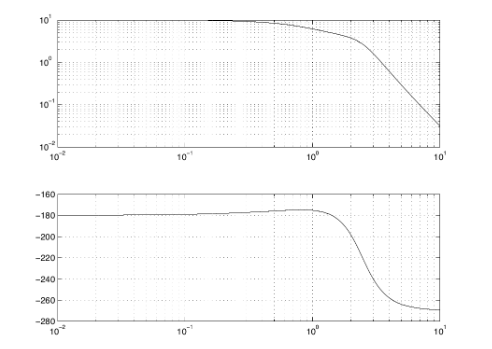
\includegraphics[width=0.6\linewidth]{./Figures/Bode_plots_for_Assignment1.png}\\
    \textbf{Fig.~1:} Bode Plot for Question~(\ref{q:bode})
  \end{center}





\begin{question}[15]
  \label{q:bode} Consider the standard feedback system with $C(s) = K$. 
  The Bode plot of $P (s)$ is given in Figure 1 (magnitude in absolute units, not dB; phase in degrees). 
  The phase starts at $-180^\circ$ and ends at $-270^\circ$. 
  You are also given that $P(s)$ has exactly one pole in the right half-plane. 
  For what range of gains $K$ is the feedback system stable?
\end{question}


\begin{solution}
  We have the fundamental equation stemming from the argument of the principle. 

  \[
     Z = N + P
  \] 

  Where 

  \begin{itemize}
    \item Z = Number of closed-loop poles in RHP
    \item N = number of CCW encirclements of -1 by the Nyqist plot $ KP(s) $
    \item P = number of open-loop poes of $ KP(s) $ in RHP  
  \end{itemize}

  Since we are given that $ P=1 $, then $ N=-1 $ must be true for our feedback system to be stable. This happens when we have a CW encirclement of the critical point. 

  From the bode plot, we see that the phase starts at $-180$ and ends at $-270$ degrees. This mean that the Nyquist curve begins on the real axis and rotates downward. At the frequency where the phase is $-180$, the magnitude determines whether the point is encircled.

  For there to be an encirclement, the point must start to the left of the critical point. i.e. when 

  \[
     K\| P(jw) \| = -1
  \] 

  \begin{itemize}
    \item For $ K < 1 $, we have $ | KP(jw) | < 1 $ and we will have no encirclements of $ -1 $
    \item For $K=1$, the Nyquist curve passes through our critical point, and we have marginal stability.
    \item For $ K > 1 $, we have that $ | KP(jw) | > 1 $ and we have an encirclement of $ -1 $
  \end{itemize}
  
  
  So for $ K > 1$, we have that $ N=-1 $ and we have 
  
  \[
     Z = (-1) + 1 = 0
  \] 
  Which from Nyquist stability criterion entails that the system is stable. The answer to the question of what range of gains K gives stability for the feedback system, the answer is that $ K > 1 $ 

\end{solution}

\question[10] Consider the feedback system:
\begin{center}
  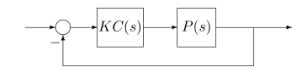
\includegraphics[width=0.5\linewidth]{Figures/feedback_system_q7.png}
\end{center}
with
\begin{align}
  P(s) =
    \dfrac{s+2}{s^2+2},~C(s) = \dfrac{1}{s}.
\end{align}

Sketch the Nyquist plot of $PC$. How many encirclements are required of the critical point for feedback stability? Determine the range of real gains $K$ for stability of the feedback system.


\begin{solution}


  $ P(s)C(s) $ is the following: 
  
  \[
     P(s)C(s) = \frac{s+2} {s^3+s} 
  \] 
  Here is the sketch of the Nyquist plot

  

  \begin{center}
    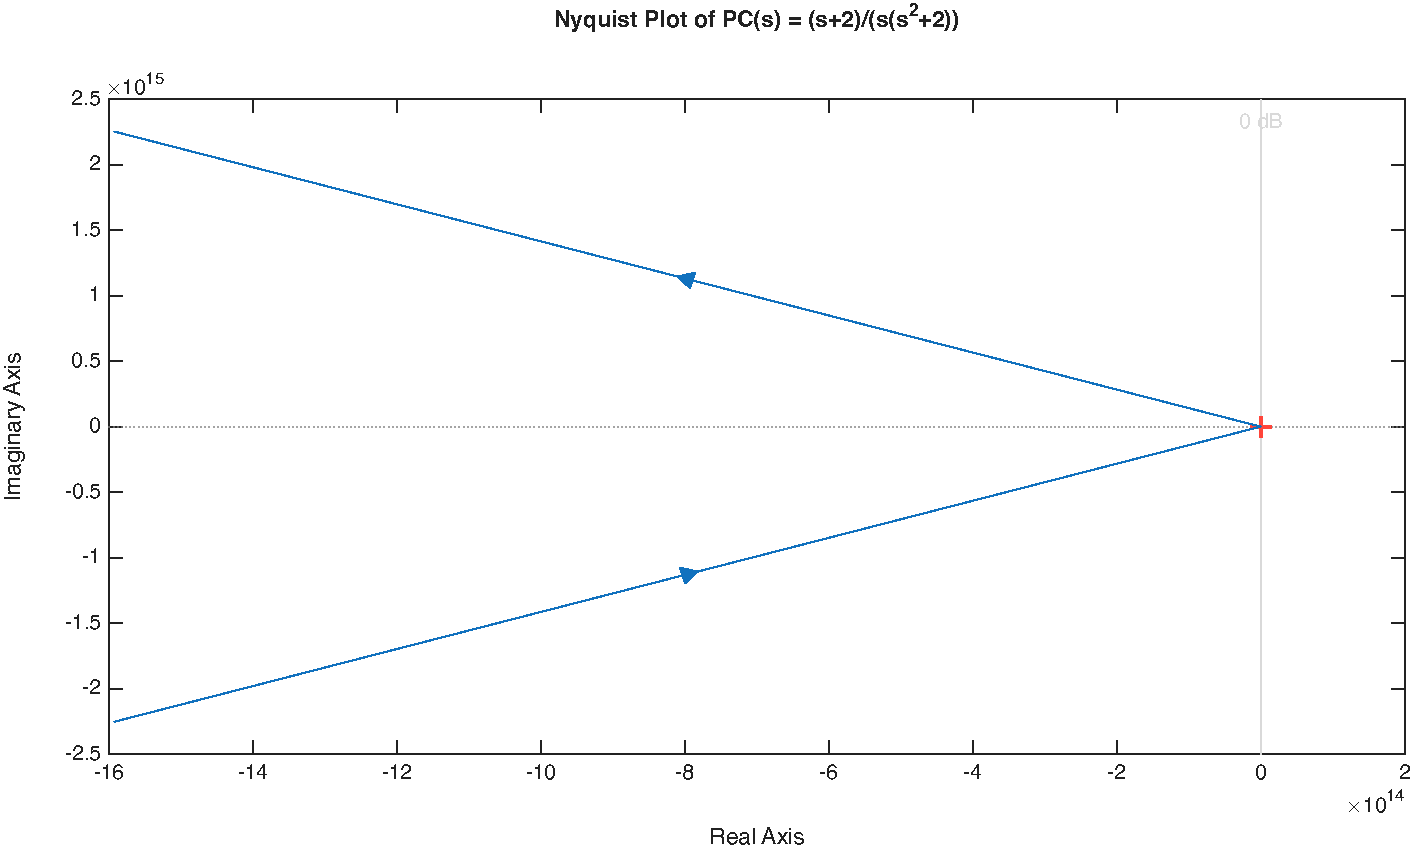
\includegraphics[width=0.8\linewidth]{Figures/nyquist_seven.pdf}
  \end{center}
  


  The denominator of PC is $ s(s^2+2) $, and the roots of this equation is
  \begin{itemize}
    \item $ 0 $ 
    \item $-\sqrt{2} i$
    \item $+\sqrt{2} i$
  \end{itemize}  

  Of which, none are in the right hand plane. Therefore, we need no encirclements of the critical point regardless if its counterclockwise or clockwise for the feedback system to be stable.


  Furthermore, we can solve for which K that gives stability, by decomposing the equation PC to a real and imaginary part, and solve for which solutions of w that gives no imaginary part. 

  \[
     L(s) = KC(s)P(s)
  \] 

  \begin{align*}
    L(s) &= \frac{K} {s} * \frac{s+2} {s^2+2} \\
    L(jw) &= \frac{K} {jw} * \frac{jw+2} {2-w^2} \\
    &= \frac{K} {2-w^2} * \left(1 - \frac{2j} {w} \right) \\
    &= \frac{K} {2-w^2} - j \left(\frac{2K} {w(2-w^2)} \right) 
  \end{align*}

  This has no finite solutions for any rational $ w $, only as w approaches $ \infty $ which means that the system is stable for all $ K>0 $ $ \frac{-1} {K}  $ is then in the LHP    
\end{solution}


\question[10]

Repeat the previous question with,
\begin{align}
  P(s) = \dfrac{s^2+1}{(s+1)(s^2+s+1)},~C(s) = 1.
\end{align}

\begin{solution}
  By plotting the nyquist curve in matlab, we get the Nyquist curve:

  \begin{center}
    
\includegraphics[width=0.8\linewidth]{Figures/nyquist_eight.pdf}
  \end{center}

  \[
     P(s) = \frac{s^2+1} {(s+1)(s^2+s+1)} 
  \] 

  This plant has poles in
  
  \begin{itemize}
    \item $ s = -1 $
    \item $ \frac{-1} {2} + \frac{j\sqrt{3}} {2}   $
    \item $ \frac{-1} {2} - \frac{j\sqrt{3}} {2}   $  
  \end{itemize}

  Since all these solutions are in the LHP, then the nyquist plot of $ P(s) $ must have no encirclements of the critical point $ \frac{-1} {K}  $ for the feedback system to be stable. By examining, if we take $ K=\frac{-1} {2}  $ for instance, we get that the critical point $ \frac{-1} {K}=2  $, which the nyquist plot does encircle at all. And for $ K>0 $ we can obviously see that this is a stable critical point. Thus, the range
  
  \[
     \left( -1, \infty \right) 
  \] 

  gives a stable feedback system
\end{solution}

\end{questions}


Here is the code for calculating the stable K range

\begin{lstlisting}[language=Matlab]

function stability_analysis_simple()
    P = tf([1 0 1], [1 2 2 1]);
    C = tf([1], [1]);

    K_min = -100;
    K_max = 100;
    n_points = abs(K_max - K_min)*1000; % More points for better numeric approximation, but this seems to do the job.
    K_values = linspace(K_min, K_max, n_points);
    
    is_stable = false(size(K_values));
    stability_boundaries = [];
    
    for i = 1:length(K_values)
        K = K_values(i);
        
        % Closed-loop system
        T = feedback(K * C * P, 1);
        is_stable(i) = isstable(T);
        
        % Detect stability boundaries (where stability changes)
        if i > 1 && is_stable(i) ~= is_stable(i-1)
            stability_boundaries = [stability_boundaries, K_values(i)];
        end
    end
    stable_indices = find(is_stable);
    
    if isempty(stable_indices)
        fprintf('No stable K values found in range [%.2f, %.2f]\n', K_min, K_max);
    else
        K_stable_min = K_values(stable_indices(1));
        K_stable_max = K_values(stable_indices(end));
        
        fprintf('\n=== STABILITY ANALYSIS RESULTS ===\n');
        fprintf('Stable range: K \in [%.4f, %.4f]\n', K_stable_min, K_stable_max);
        fprintf('Stability boundaries found at: ');
        if ~isempty(stability_boundaries)
            fprintf('K = %.4f', stability_boundaries(1));
            for j = 2:length(stability_boundaries)
                fprintf(', K = %.4f', stability_boundaries(j));
            end
            fprintf('\n');
        else
            fprintf('None detected in tested range\n');
        end
        fprintf('Number of stable K values: %d/%d\n', sum(is_stable), length(K_values));
    end
    
    % Plot the stability results
    figure;
    stem(K_values, is_stable, 'filled', 'MarkerSize', 2);
    xlabel('Gain K');
    ylabel('Stability (1 = Stable, 0 = Unstable)');
    title('Stability vs Gain K');
    grid on;
    ylim([-0.1 1.1]);
    
    % Highlight stable region
    if ~isempty(stable_indices)
        hold on;
        area(K_values(stable_indices), ones(size(stable_indices)), ...
            'FaceColor', 'g', 'FaceAlpha', 0.2, 'EdgeColor', 'none');
        hold off;
        legend('Stability', 'Stable Region', 'Location', 'best');
    end
    
    % Test and display a few specific points for verification
    fprintf('\n=== VERIFICATION AT SPECIFIC POINTS ===\n');
    test_points = unique([K_min, K_stable_min, 0, K_stable_max, K_max, stability_boundaries]);
    test_points = test_points(isfinite(test_points));
    
    for i = 1:min(6, length(test_points)) % Show up to 6 points
        K = test_points(i);
        T = feedback(K * C * P, 1);
        poles = pole(T);
        
        fprintf('K = %7.3f: ', K);
        if isstable(T)
            fprintf('STABLE   ');
        else
            fprintf('UNSTABLE ');
        end
        fprintf('Poles: ');
        for j = 1:min(3, length(poles)) % Show up to 3 poles
            fprintf('%.3f%+.3fi ', real(poles(j)), imag(poles(j)));
        end
        if length(poles) > 3
            fprintf('...');
        end
        fprintf('\n');
    end
end

stability_analysis_simple()


%% 


% Helper function for detailed analysis at specific K values
function analyze_specific_K(num_P, den_P, num_C, den_C, K_values)
    % Precompute the polynomial components
    den_product = conv(den_P, den_C);
    num_product = conv(num_P, num_C);
    
    % Ensure both polynomials have the same length
    max_length = max(length(den_product), length(num_product));
    den_product_padded = [zeros(1, max_length - length(den_product)), den_product];
    num_product_padded = [zeros(1, max_length - length(num_product)), num_product];
    
    for K = K_values
        fprintf('\n=== Detailed Analysis for K = %.4f ===\n', K);
        
        % Form the characteristic polynomial
        char_poly = den_product_padded + K * num_product_padded;
        
        % Find roots
        r = roots(char_poly);
        
        % Display results
        fprintf('Characteristic polynomial: ');
        % Create a nice string representation
        poly_str = '';
        for j = 1:length(char_poly)
            if char_poly(j) ~= 0
                if j == 1
                    poly_str = sprintf('%.4f', char_poly(j));
                else
                    exponent = length(char_poly) - j;
                    if exponent == 1
                        poly_str = sprintf('%s + %.4fs', poly_str, char_poly(j));
                    else
                        poly_str = sprintf('%s + %.4fs^%d', poly_str, char_poly(j), exponent);
                    end
                end
            end
        end
        disp(poly_str);
        
        fprintf('Roots:\n');
        for j = 1:length(r)
            fprintf('  s%d = %.4f %+.4fi\n', j, real(r(j)), imag(r(j)));
        end
        
        % Check stability
        if all(real(r) < 0)
            fprintf('SYSTEM IS STABLE\n');
        else
            fprintf('SYSTEM IS UNSTABLE\n');
        end
    end
end



% Optional: Analyze specific points of interest
analyze_specific_K([1, 0, 1], [1, 2, 2, 1], [1], [1, 0], 1);

\end{lstlisting}


\end{document}